\documentclass[../main.tex]{subfiles}
\graphicspath{{\subfix{../images/}}}
\begin{document}



\begin{lemma}[O zaplnění]
    Nechť \matAsquare je SPD, $i,j\in \hat{n}, i>j, k\in \hat{n}$.\\
    Potom $a_{ij}^{(k)} \neq 0 \Leftrightarrow a_{ij}^{(k-1)} \neq 0$ nebo $a_{ik}^{(k-1)} \neq 0 \wedge a_{kj}^{(k-1)} \neq 0$
\end{lemma}

\begin{proof}
    Aby prvek v kroku $k$ byl nenulový, tak musel buď být nenulový v minulém kroku nebo vznikne násobením právě těchto dvou prvků.
\end{proof}

\begin{theorem}[O zaplnění]
    Nechť \matAsquare je SPD,$i,j\in \hat{n}, i>j$.\\
    Potom $a_{ij}^{(n-1)} \neq 0 \Leftrightarrow \exists$ cesta v $G(\mathbf{A})$, $i,p_1,p_2... p_t,j$ kde $\forall k \in \hat{t}, p_k < j$.
\end{theorem}

\begin{proof}
    $(\implies)$

    Dokazujeme indukcí podle $j$: \\$j=1$:$ a_{ij}^{(n-1)} \neq 0 \Leftrightarrow a_{ij}^{(0)} \neq 0 \Leftrightarrow (i,1)\in E$.

    Předpokládáme, že platí pro $j-1$.

    \begin{center}
        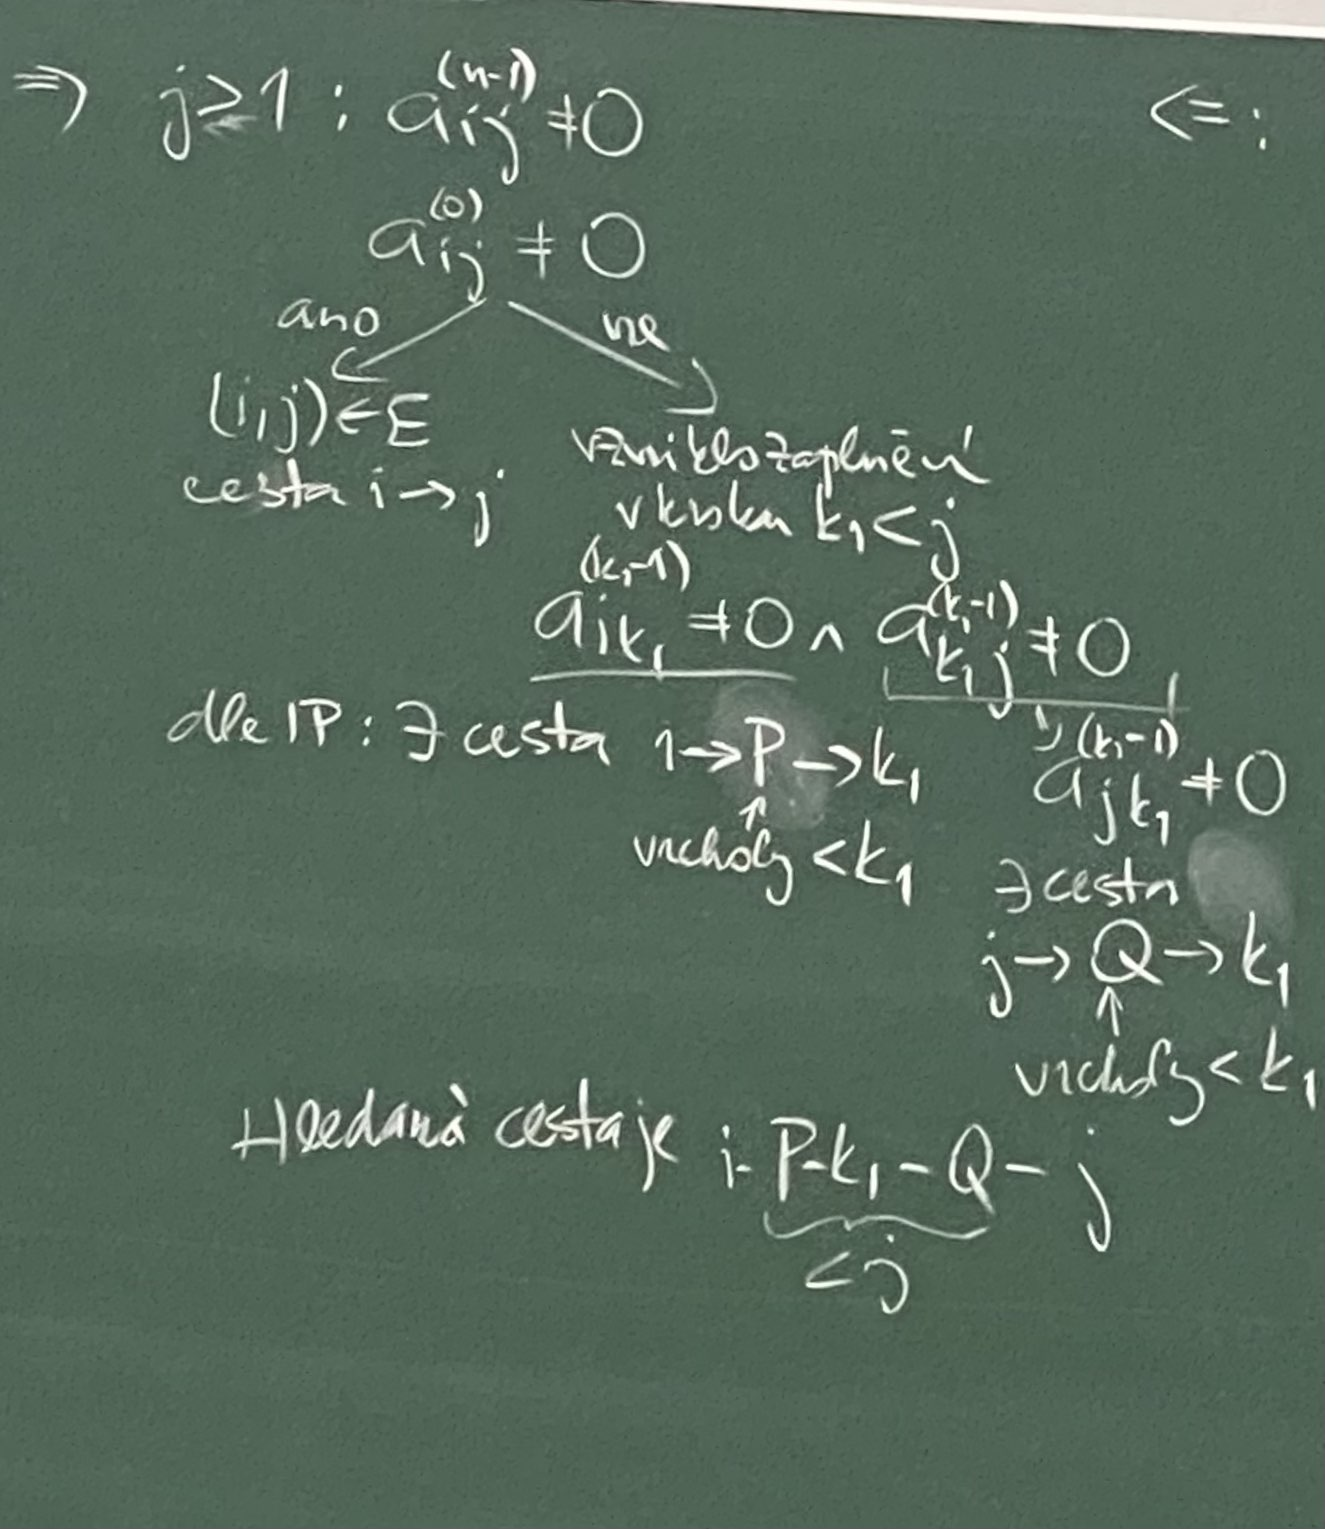
\includegraphics[width=0.5\linewidth]{images/19-10-dukazzleva.jpg}
    \end{center}

    $(\impliedby)$ 
    
    Při eliminaci například $p_1$ z $G(\mathbf{A})$ vznikne 
    hrana $i\rightarrow p_2$. Při eliminaci vrcholu se cesta 
    z $i \rightarrow j$ vedoucí přes $p_1,...,p_t$ zkrátí 
    alespoň o 1.

    $p_1 ... p_t$ se eliminují před $j$ a $i$. Po eliminaci 
    posledního z $p_1,...,p_t$ se $i$ a $j$ spojí hranou

    Z toho víme, že na pozici $a_ij$ vzniká zaplnění $\implies a_{ij}^{(n-1)}\neq 0$.
\end{proof}

\subsection{Eliminační strom}

Eliminační strom matice $\mathbf{L}$ 
(pocházející z Choleského faktorizace SPD matice \matAsquare) 
je $T = (V, E_T)$, kde $V=\hat{n}$ a předek $[j] = \min \{i\in\hat{n} \mid e_{ij} \neq 0, i>j \}$, tj. 
$(i,j) \in E_T \Leftrightarrow e_{ij} \neq 0 \wedge e_{kj} = 0$

\begin{equation*}
    \mathbf{A} = \begin{bmatrix}
        \times &  &  & \times &  \\
         & \times &  &  & \times \\
         &  & \times & \times & \times \\
        \times &  & \times & \times &  \\
         & \times & \times &  & \times 
        \end{bmatrix}  \rightarrow
        \mathbf{L} + \hat{\mathbf{L}} = 
        \begin{bmatrix}
            \times &  &  & \times &  \\
             & \times &  &  & \times \\
             &  & \times & \times & \times \\
            \times &  & \times & \times & z \\
             & \times & \times & z & \times 
            \end{bmatrix} 
\end{equation*}

Eliminační stromy se definují na základě struktury matice \matL , ne \matA . 

\subsubsection{Vlastnosti eliminačních stromů}
\begin{claim}
Kořenem eliminačního strom je vrchol s největším indexem
\end{claim}

\begin{claim}
$i$ je předkem $j$ v $T \implies i> j $
\end{claim}

\begin{claim}
$e_{ij}\neq 0$ pro $i>j \implies i$ je předkem $j$ v $T$
\end{claim}
\begin{proof}
    \hphantom{text}

        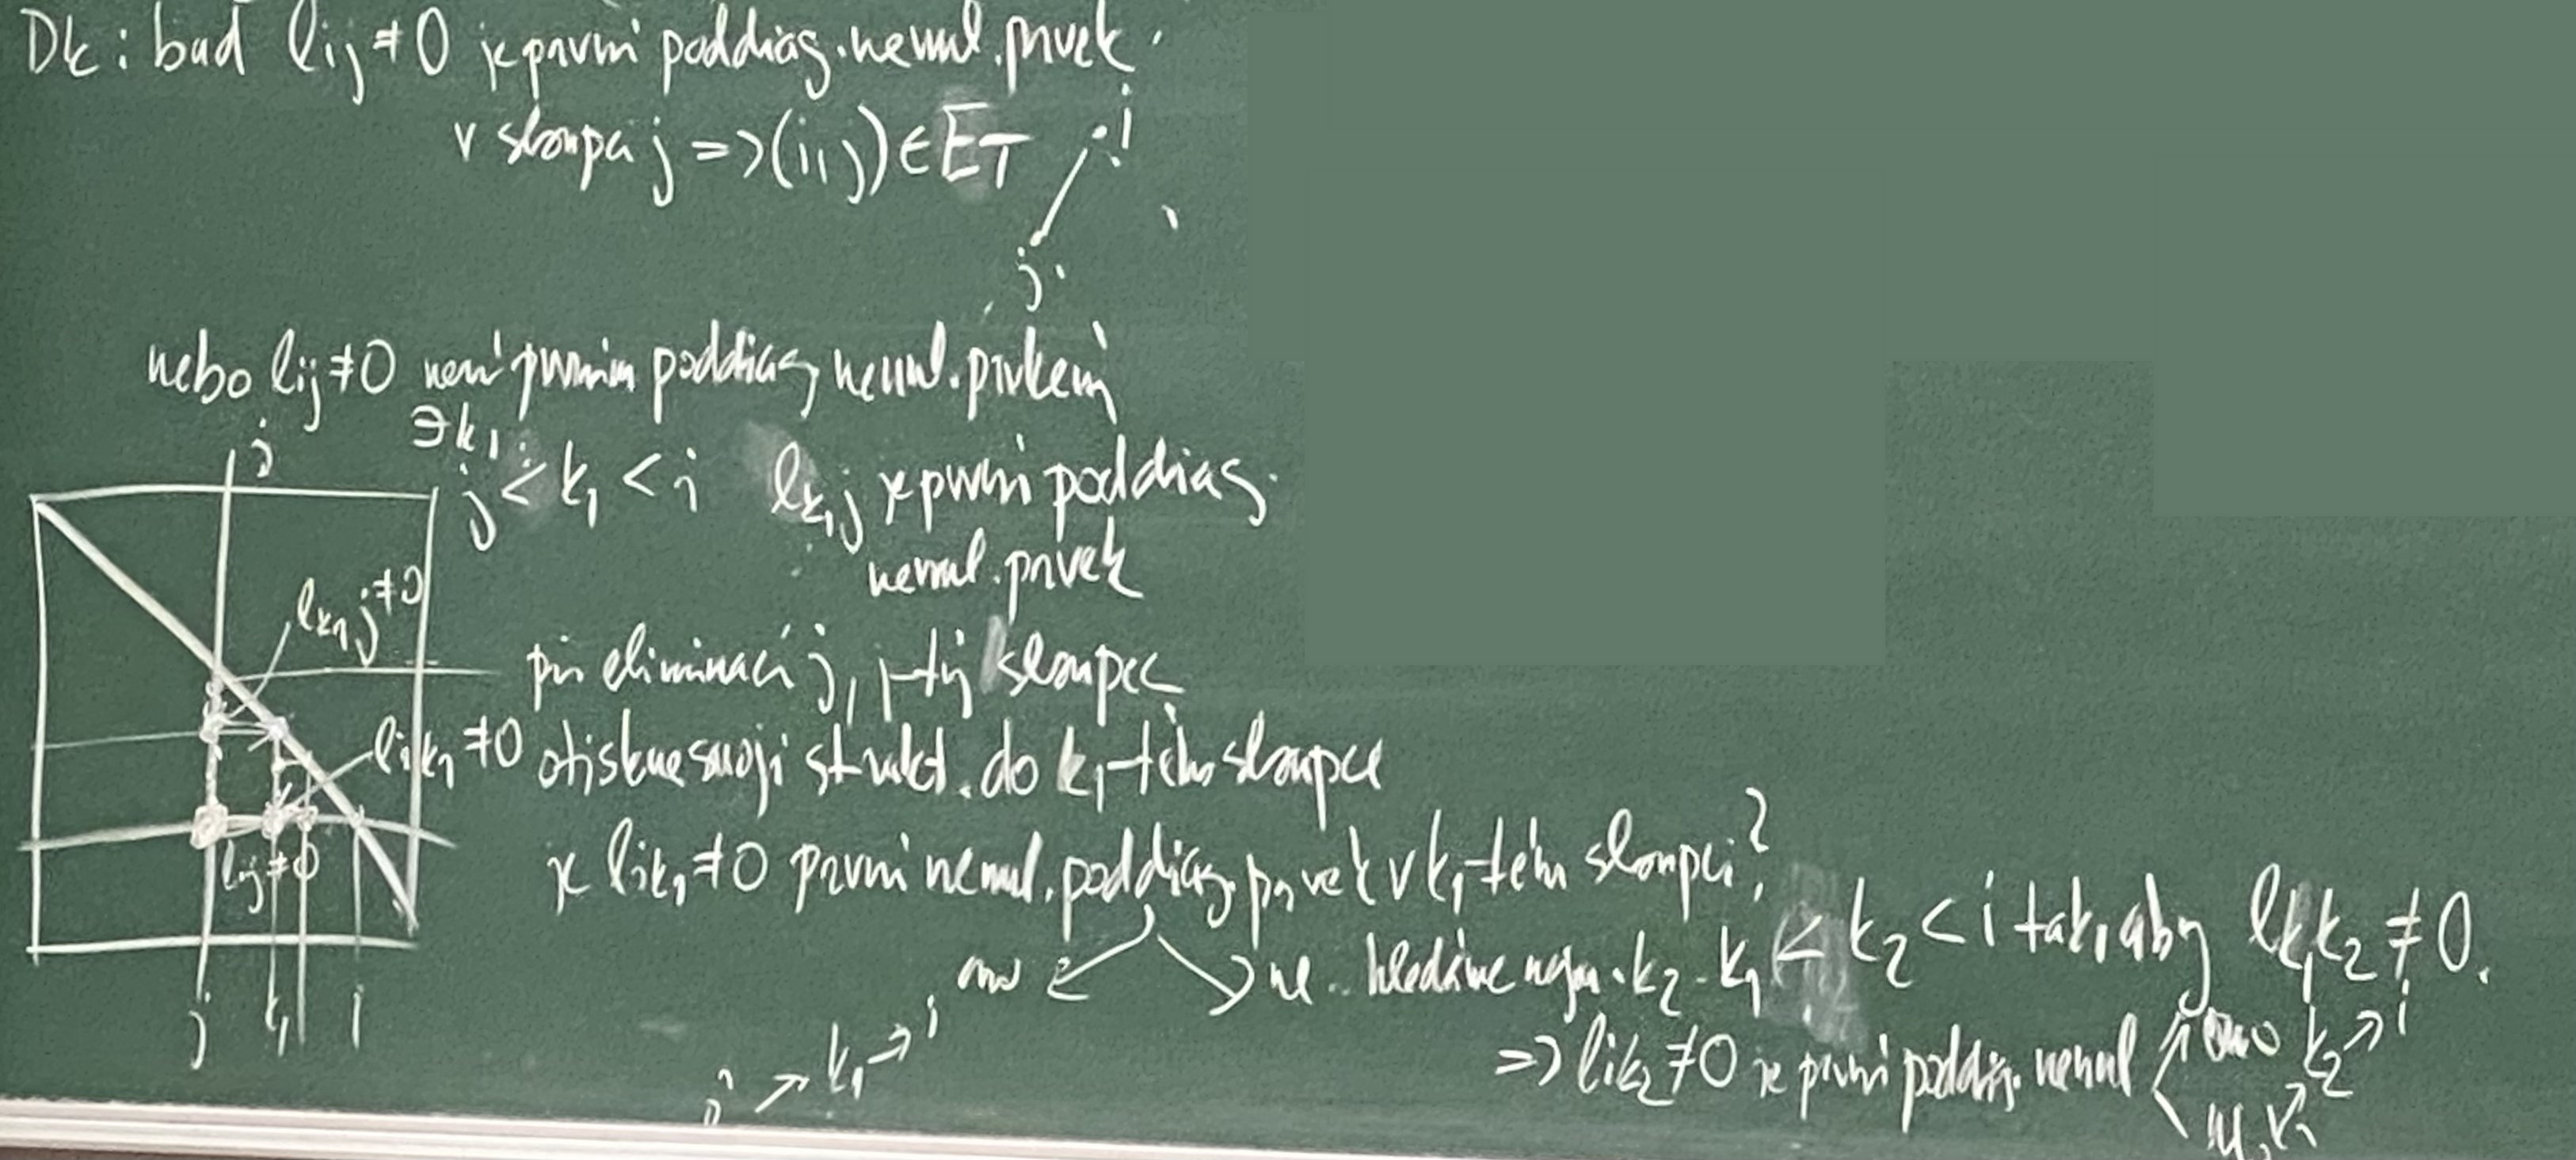
\includegraphics[width=0.9\linewidth]{images/19-10-dukaz2.jpg}
\end{proof}

\begin{remark}
    Tuto implikaci nelze obrátit.
\end{remark}
\begin{claim}
Jsou-li $T_i$ a $T_j$ disjunktní podstromy eliminačního stromu s kořeny ve vrcholech $i$, respektive $j$,
pak $\forall r \in T_i$ a $s\in T_j$ platí $e_{rs} = 0$
\end{claim}
\begin{proof}
    Negace předchozího tvrzení. 
\end{proof}


\begin{claim}
    Nechť \matAsquare je SPD, $i,j\in\hat{n}, i>j$.\\
    Potom $e_{ij} \neq 0 \Leftrightarrow j$ je předek 
    nějakého $k$, pro dané $a_{ik}^{(0)}\neq 0$.
\end{claim}
\begin{proof}
    \hphantom{text}

    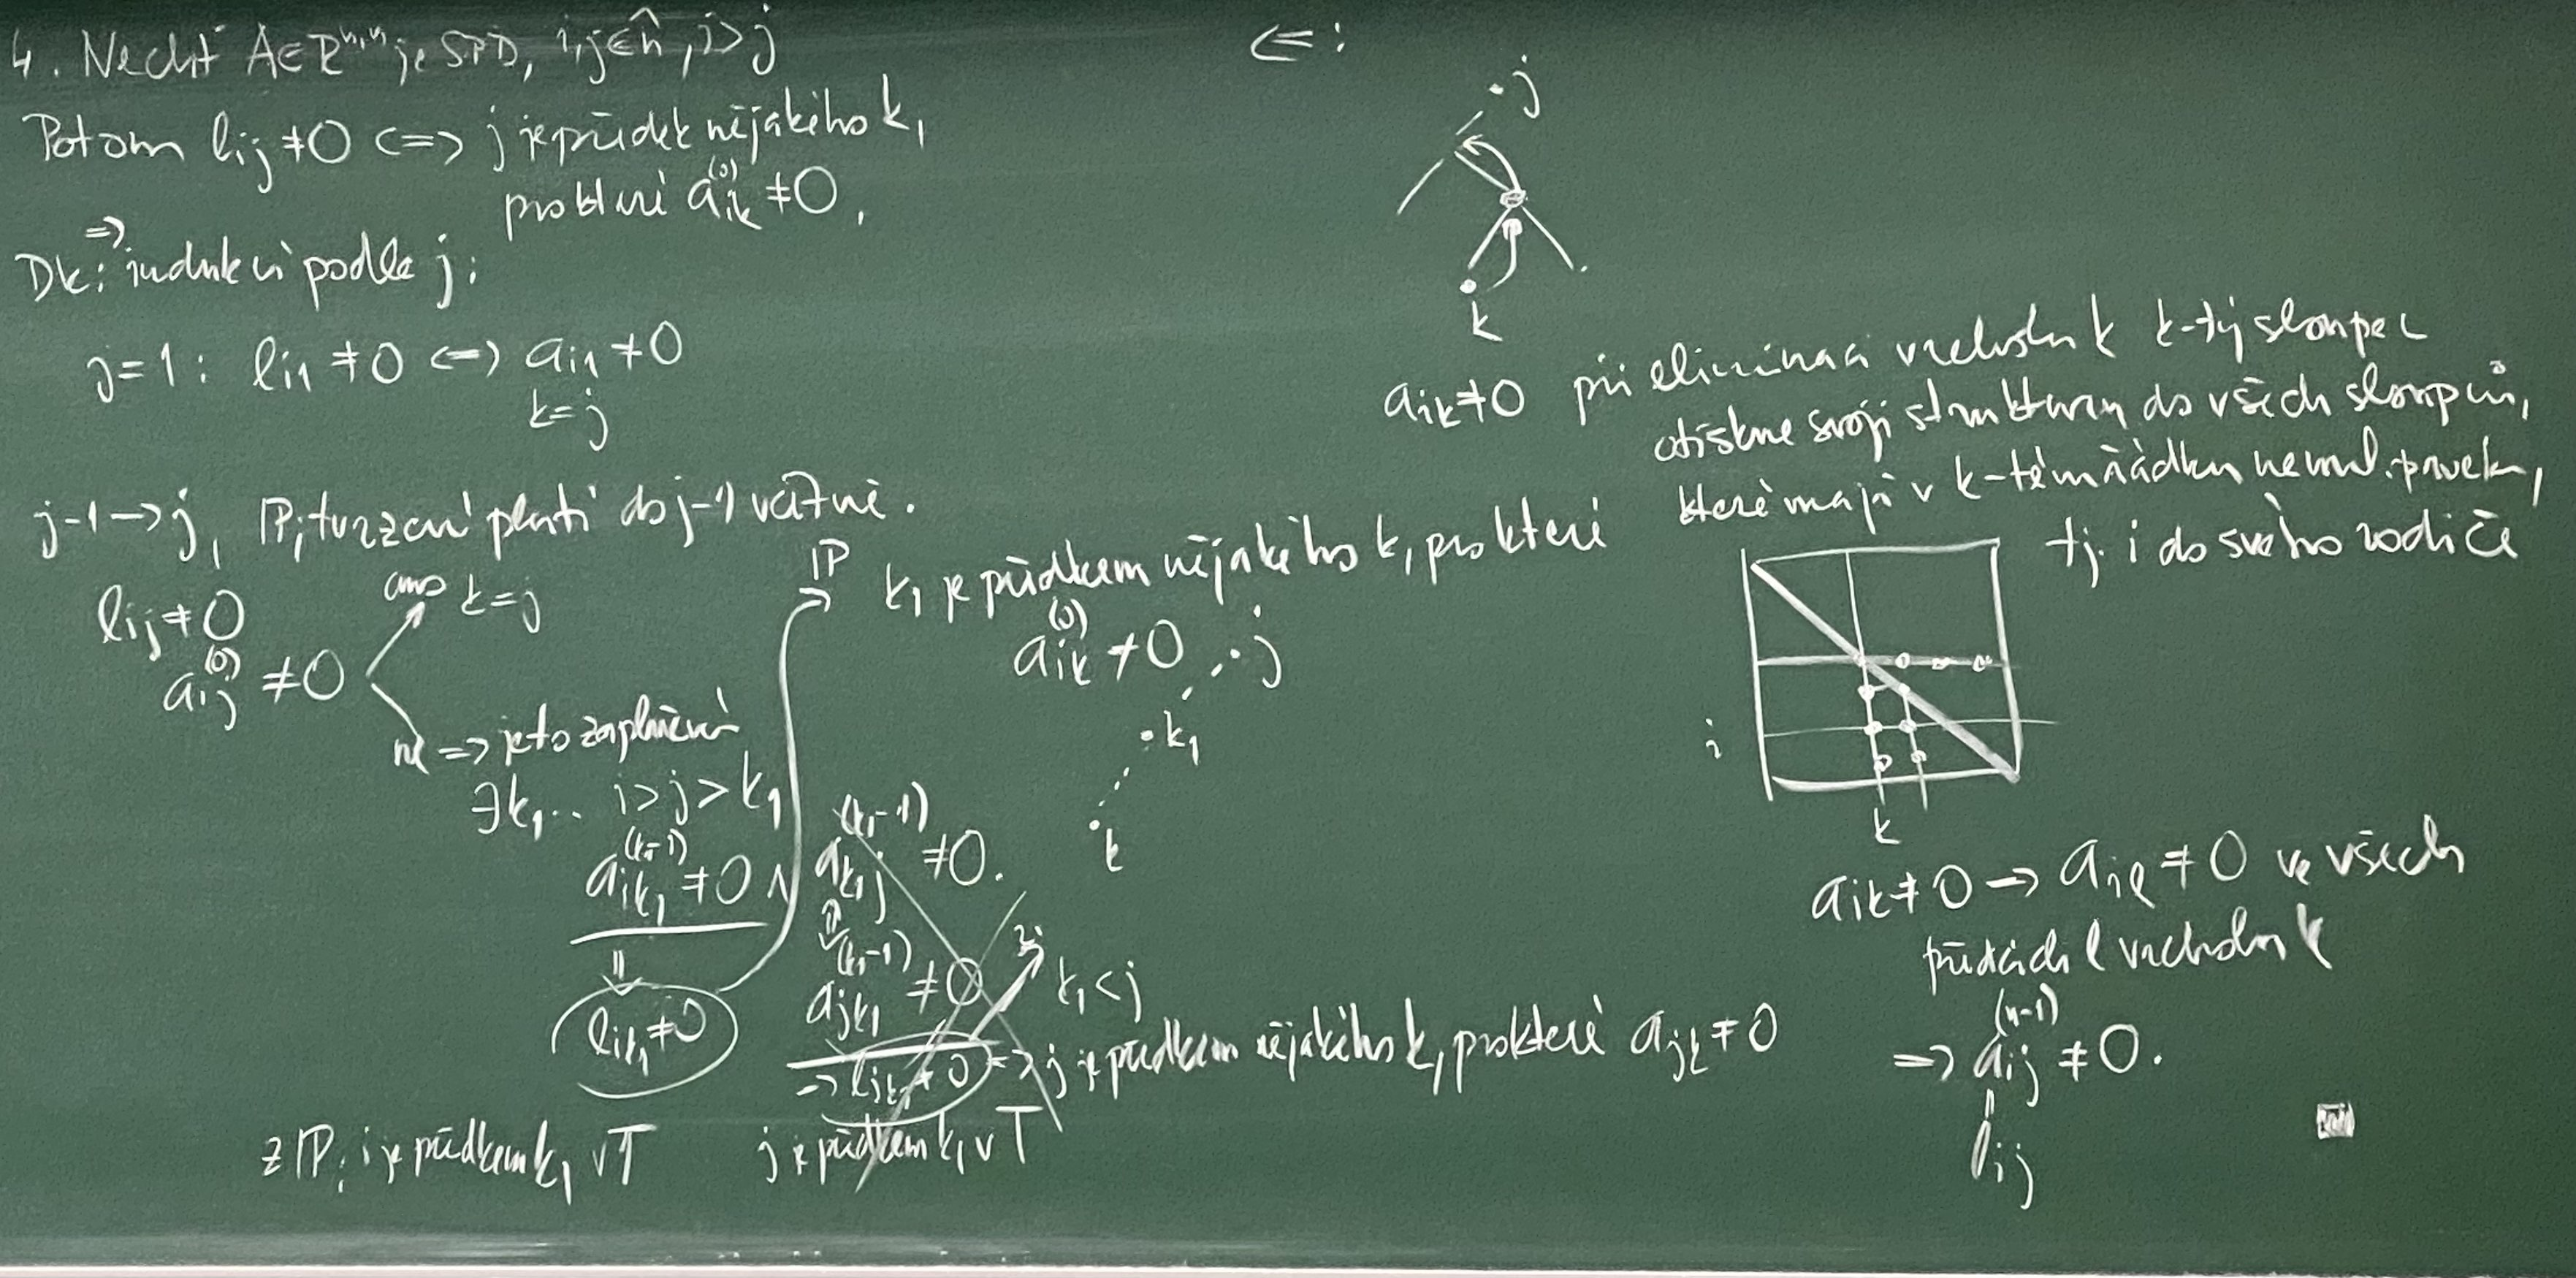
\includegraphics[width=0.9\linewidth]{images/19-10-dukaz4.jpg}
\end{proof}


\begin{corollary}
    Strukturu matice \matL lze odvodit z eliminačního stromu a struktury matice \matA . 

    Nenulové prvky v $i$-tém řádku matice \matL (struktura $i$-tého řádku) jsou právě
    ty prvky v $T_i$ ležící na cestě mezi $i$ a nějakým $k$, pro které $a_{ik} \neq 0$.
\end{corollary}

\begin{definition}
    $Struct(\mathbf{L}, j) - \left\{  i\in \hat{n}\mid e_{ij} \neq 0, i>j \right\}$
\end{definition}

\begin{theorem}
    $Struct(L,j) = Struct(A,j) \cup \bigcup_{k\in T_j} Struct (L, k)\setminus \widehat{j-1}$
\end{theorem}

\begin{proof}
    Z obrázku

    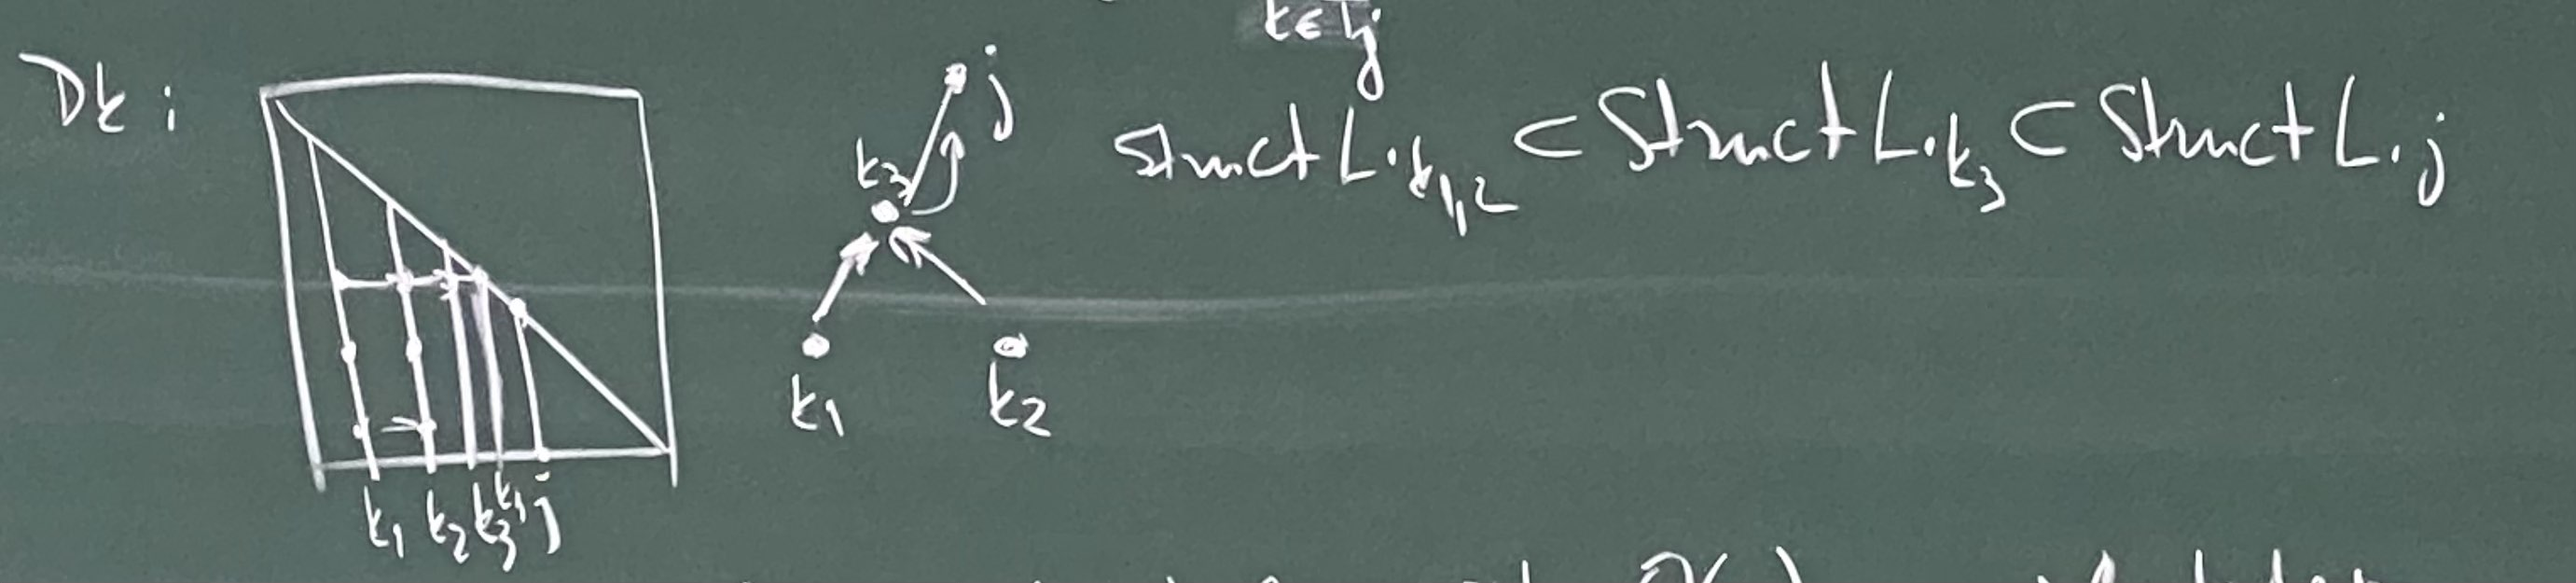
\includegraphics[width=0.9\linewidth]{images/19-10-dukazfinal.jpg}
\end{proof}



$\implies$ strukturu sloupců matice \matL lze určit v $O(m)$ operacích, kde $m$ je počet nenulových prvků matice \matL . 
















\end{document}